\section{Methodologies under Comparison}
\label{sec:methodology}

\begin{figure*}[t]
\centering
\begin{tikzpicture}[
    node distance=0.85cm and 0.9cm,
    every node/.style={font=\footnotesize},
    block/.style={rectangle, draw=black!70, rounded corners=3pt, fill=blue!5, text width=2.4cm, minimum height=0.9cm, align=center, line width=0.6pt},
    baseline/.style={rectangle, draw=teal!80, rounded corners=3pt, fill=teal!6, text width=2.4cm, minimum height=0.9cm, align=center, line width=0.6pt},
    eval/.style={rectangle, draw=orange!80, rounded corners=3pt, fill=orange!8, text width=2.3cm, minimum height=0.9cm, align=center, line width=0.6pt},
    source/.style={rectangle, draw=gray!80, rounded corners=3pt, fill=gray!10, text width=3.0cm, minimum height=0.7cm, align=center, font=\footnotesize\bfseries},
    arrow/.style={-Latex, thick, draw=black!70},
    dashedarrow/.style={-Latex, dashed, thick, draw=black!60}
]

% Source
\node[source] (textbook) {Source Textbook\\(\texttt{CK-12 Basic Geometry})};

% Preprocessing
\node[block, below=0.6cm of textbook, text width=5.5cm] (preprocess) {
    \textbf{Text Ingestion \& Preprocessing}\\
    Structure Detection (Def, Thm, Expl) \& Segmentation
};

% Pipelines
\node[block, below left=0.9cm and 0.4cm of preprocess, text width=3.4cm, fill=purple!6, draw=purple!80] (rule_pipe) {
    \textbf{Rule Pipeline (\texttt{rule\_v3})}\\
    \textit{Lexicon:} 130 Curated Concepts\\
    \textit{Pairs:} Intra-sentence cooc\\
    \textit{Classify:} Hearst \& Connectives\\
    \textit{Score:} Saaty AHP ($CR=0.022$)
};

\node[block, below right=0.9cm and 0.4cm of preprocess, text width=3.4cm, fill=red!6, draw=red!80] (llm_pipe) {
    \textbf{LLM Pipeline (\texttt{kgx\_v2})}\\
    \textit{Concepts:} spaCy Noun Chunks (204)\\
    \textit{Pairs:} Multi-source (989 pairs)\\
    \textit{Classify:} Swap-sampled 7B Prompt\\
    \textit{Constraint:} Feedback Arc Set
};

% Baselines & Hybrid
\node[baseline, left=0.6cm of rule_pipe, text width=2.5cm] (book_order) {
    \textbf{Reading Order Prior}\\
    \textit{Rule:} $p(A) < p(B)$\\
    \textit{Score:} $\Delta \text{Position}$
};

\node[block, below=0.9cm of llm_pipe, text width=3.6cm, fill=green!6, draw=green!70!black] (hybrid_pipe) {
    \textbf{Neuro-Symbolic Hybrid}\\
    \textit{Expansion:} Cartesian ($N=41{,}412$)\\
    \textit{Gate:} Forward Order $\times$ Rank Fusion\\
    \textit{Acyclicity:} Topological DAG Sorting
};

% Evaluation
\node[eval, below=1.2cm of rule_pipe, text width=2.8cm] (eval_rule) {
    \textbf{Evaluation on Gold}\\
    AL-CPL Benchmark\\
    Direct $F_1 = 0.052$\\
    $\text{AUC} = 0.513$
};

\node[eval, below=1.2cm of hybrid_pipe, text width=2.8cm] (eval_hybrid) {
    \textbf{Evaluation on Gold}\\
    AL-CPL Benchmark\\
    Closure $F_1 = 0.786$\\
    $\text{AUC} = 0.888$
};

\node[eval, below=1.2cm of book_order, text width=2.5cm] (eval_order) {
    \textbf{Structural Baseline}\\
    Direct $F_1 = 0.736$\\
    $\text{AUC} = 0.868$\\
    Acc $= 96.5\%$
};

\node[eval, below=0.4cm of llm_pipe, text width=3.2cm, fill=red!10, draw=red!70] (eval_llm) {
    \textbf{LLM Directional Score}\\
    Direct $F_1 = 0.030$, $\text{AUC} = 0.503$\\
    Directional Acc $= 50.0\%$ (Chance)
};

% Connectors
\draw[arrow] (textbook) -- (preprocess);
\draw[arrow] (preprocess.south) -| (rule_pipe.north);
\draw[arrow] (preprocess.south) -| (llm_pipe.north);
\draw[dashedarrow] (preprocess.west) -| (book_order.north);

\draw[arrow] (llm_pipe.south) -- (eval_llm.north);
\draw[dashedarrow] (llm_pipe.south) -- (hybrid_pipe.north);
\draw[dashedarrow] (book_order.south) |- ($(hybrid_pipe.west)+(0,0.2)$);

\draw[arrow] (rule_pipe.south) -- (eval_rule.north);
\draw[arrow] (hybrid_pipe.south) -- (eval_hybrid.north);
\draw[arrow] (book_order.south) -- (eval_order.north);

\end{tikzpicture}
\caption{System architecture and comparative evaluation workflow across the three knowledge graph construction pipelines (\texttt{rule\_v3}, \texttt{kgx\_v2}, \texttt{kgx\_v2\_hybrid}) and the structural reading-order baseline, evaluated against the external AL-CPL benchmark on identical covered candidate pairs.}
\label{fig:methodology_flowchart}
\end{figure*}

\begin{table*}[t]
\centering
\small
\caption{Systematic methodology comparison across evaluated educational knowledge graph construction pipelines, structural baselines, and feature weighting ablations.}
\label{tab:methodology_comparison}
\begin{tabularx}{\textwidth}{l p{2.4cm} p{2.2cm} p{2.4cm} p{2.2cm} p{2.5cm} l}
\toprule
\textbf{Approach} & \textbf{Paradigm} & \textbf{Concept Extraction} & \textbf{Candidate Pairing} & \textbf{Direction Decided By} & \textbf{Graph Constraints} & \textbf{Runtime} \\
\midrule
\multicolumn{7}{l}{\textit{\textbf{Group A: End-to-End Construction Pipelines}}} \\
\addlinespace[2pt]
\texttt{rule\_v3} & Heuristic / Symbolic Regex & Hard-coded lexicon (130 nodes) & Intra-sentence co-occurrence only & Passive voice cues or reading-order fallback & Manual deduplication; cycles unconstrained & $\approx 8.4$\,s \\
\addlinespace[3pt]
\texttt{kgx\_v2} & Open-weight Local LLM (\texttt{Qwen-2.5-7B}) & Unsupervised spaCy discovery (204 nodes) & Multi-source proposal (cooc, embeddings) & Swap-sampled zero-shot JSON prompting & Greedy feedback arc set (DAG on Prereq) & $\approx 68$\,m \\
\addlinespace[3pt]
\texttt{kgx\_v2\_hybrid} & Neuro-Symbolic Synthesis & Inherits 204 nodes from \texttt{kgx\_v2} & Cartesian candidate expansion ($N=41{,}412$) & Forward reading gate ($p_A < p_B$) $\times$ rank fusion & Strict DAG on Prereq; top-$3$ predecessor bound & $\approx 22$\,s \\
\midrule
\multicolumn{7}{l}{\textit{\textbf{Group B: Comparative Baselines}}} \\
\addlinespace[2pt]
Random & Non-informative baseline & N/A & Evaluated candidate pairs & Uniform random assignment & None & $< 0.1$\,s \\
\addlinespace[3pt]
Book Order & Zero-parameter structural prior & Offset scanning of textbook text & All covered candidate pairs ($N=868$) & First-mention offset in raw text: $p(A) < p(B)$ & Inherently acyclic (transitive linear chain) & $< 0.5$\,s \\
\midrule
\multicolumn{7}{l}{\textit{\textbf{Group C: Edge Weighting \& Scoring Ablations (Prerequisite Ranking)}}} \\
\addlinespace[2pt]
Saaty AHP & Multi-Criteria Decision Analysis & Verified first definitions & Evaluated candidate pairs & Symmetric: $W(A,B) = W(B,A)$ (No direction) & Normalized weights $W \in [0, 1]$ & $< 1.0$\,s \\
Co-occurrence & Distributional statistical count & Sentence token sets & Evaluated candidate pairs & Symmetric: $C(A,B) = C(B,A)$ (No direction) & Linear frequency saturation $\min(1, n/3)$ & $< 0.2$\,s \\
\bottomrule
\end{tabularx}
\end{table*}


We evaluate three complete knowledge graph construction pipelines, one structural baseline, and one statistical reference baseline. Figure~\ref{fig:methodology_flowchart} illustrates the system architecture, Table~\ref{tab:methodology_comparison} summarizes their methodological properties, and Figure~\ref{fig:methodology_comparison} contrasts their information sources.

\begin{figure}[t]
\centering
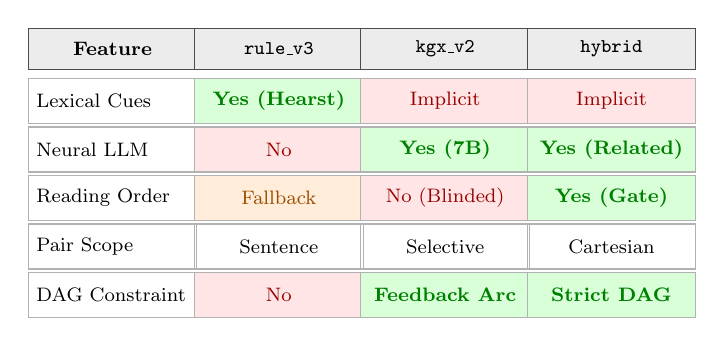
\begin{tikzpicture}[
    scale=0.88, every node/.style={transform shape, font=\footnotesize},
    header/.style={rectangle, draw=black!70, fill=gray!15, text width=2.2cm, align=center, font=\footnotesize\bfseries, minimum height=0.6cm},
    cell/.style={rectangle, draw=black!30, text width=2.2cm, align=center, minimum height=0.65cm},
    yesnode/.style={cell, fill=green!15, text=green!50!black, font=\footnotesize\bfseries},
    nonode/.style={cell, fill=red!10, text=red!60!black},
    partnode/.style={cell, fill=orange!15, text=orange!60!black}
]

% Headers
\node[header] (h0) at (0,0) {Feature};
\node[header] (h1) at (2.4,0) {\texttt{rule\_v3}};
\node[header] (h2) at (4.8,0) {\texttt{kgx\_v2}};
\node[header] (h3) at (7.2,0) {\texttt{hybrid}};

% Row 1: Explicit Cues
\node[cell, align=left] (r10) at (0,-0.75) {Lexical Cues};
\node[yesnode] (r11) at (2.4,-0.75) {Yes (Hearst)};
\node[nonode] (r12) at (4.8,-0.75) {Implicit};
\node[nonode] (r13) at (7.2,-0.75) {Implicit};

% Row 2: Neural Semantics
\node[cell, align=left] (r20) at (0,-1.45) {Neural LLM};
\node[nonode] (r21) at (2.4,-1.45) {No};
\node[yesnode] (r22) at (4.8,-1.45) {Yes (7B)};
\node[yesnode] (r23) at (7.2,-1.45) {Yes (Related)};

% Row 3: Reading Order
\node[cell, align=left] (r30) at (0,-2.15) {Reading Order};
\node[partnode] (r31) at (2.4,-2.15) {Fallback};
\node[nonode] (r32) at (4.8,-2.15) {No (Blinded)};
\node[yesnode] (r33) at (7.2,-2.15) {Yes (Gate)};

% Row 4: Candidate Pairing
\node[cell, align=left] (r40) at (0,-2.85) {Pair Scope};
\node[cell] (r41) at (2.4,-2.85) {Sentence};
\node[cell] (r42) at (4.8,-2.85) {Selective};
\node[cell] (r43) at (7.2,-2.85) {Cartesian};

% Row 5: Graph Constraints
\node[cell, align=left] (r50) at (0,-3.55) {DAG Constraint};
\node[nonode] (r51) at (2.4,-3.55) {No};
\node[yesnode] (r52) at (4.8,-3.55) {Feedback Arc};
\node[yesnode] (r53) at (7.2,-3.55) {Strict DAG};

\end{tikzpicture}
\caption{Information sources and inductive constraints across the three construction pipelines.}
\label{fig:methodology_comparison}
\end{figure}



\subsection{Method 1: Rule-Based Pipeline (\texttt{rule\_v3})}
The symbolic pipeline implements deterministic information extraction anchored in textbook structural hierarchy:
\begin{enumerate}[leftmargin=*]
    \item \textbf{Text Parsing and Structure Detection:} The document is parsed into $72$ structured blocks classified into didactic types (\textit{Definition}, \textit{Theorem}, \textit{Explanation}, \textit{Chapter}, \textit{Section}) using pattern-based structural heuristics.
    \item \textbf{Curated Lexicon Grounding:} Concepts are matched against a curated textbook vocabulary of $130$ canonical mathematical entities. Surface forms are normalized using alias maps, and first definitions are captured verbatim. Acronyms shorter than three characters are excluded.
    \item \textbf{Intra-Sentence Candidate Pairing:} Candidate relation pairs are proposed strictly when two concepts co-occur within the same sentence or definition clause ($192$ total proposals). Concepts in distinct chapters cannot form candidate pairs unless explicitly co-mentioned.
    \item \textbf{Linguistic Pattern Extraction:} Rules match curated connective regexes (\texttt{KEYWORD\_RES}) and Hearst patterns (\texttt{ONTOLOGY\_PATTERNS}). Prerequisite direction is assigned via passive-voice inversion cues or falls back to textbook sequence.
    \item \textbf{Saaty AHP Edge Weighting:} Edge confidence is calculated via the Analytic Hierarchy Process ($CR=0.022$):
    \begin{equation}
    W_{\text{AHP}} = 0.52 S + 0.24 C + 0.09 P + 0.15 E
    \end{equation}
    where $S$ is lexical definition Jaccard, $C = \min(1.0, n_{\text{sentences}}/3)$ is co-occurrence frequency, $P = 1 / (1 + |\text{chap}_A - \text{chap}_B|)$ is chapter proximity, and $E$ is section co-mention overlap.
\end{enumerate}

\subsection{Method 2: Standalone Local LLM Pipeline (\texttt{kgx\_v2})}
The neural pipeline implements open-weight generative extraction without pre-compiled lexicons:
\begin{enumerate}[leftmargin=*]
    \item \textbf{Unsupervised Concept Discovery:} The raw text is segmented into $1{,}200$-token windows. Noun chunks are extracted via spaCy and filtered by document frequency and capitalization thresholds, discovering $204$ canonical concepts.
    \item \textbf{Multi-Source Candidate Proposal:} To capture cross-chapter dependencies, candidates are generated across four channels: sentence co-occurrence, chunk co-occurrence, definition cross-references, and embedding nearest neighbors ($989$ proposed candidate pairs).
    \item \textbf{Swap-Sampled Generative Classification:} For each candidate pair $(u, v)$, the local open-weight model (\texttt{Qwen-2.5-7B-Instruct} via Ollama) is queried with the surrounding text context. To cancel positional framing bias, the model is queried twice with swapped arguments—$(u, v)$ and $(v, u)$—and the resulting JSON probability distributions across the five relation classes are averaged.
    \item \textbf{DAG Cycle Elimination:} A greedy feedback arc set algorithm detects and removes cycles on Prerequisite edges, guaranteeing an acyclic prerequisite subgraph ($545$ total multi-relation edges).
\end{enumerate}

\subsection{Method 3: Neuro-Symbolic Hybrid (\texttt{kgx\_v2\_hybrid})}
The hybrid system synthesizes neural relatedness with structural text priors:
\begin{enumerate}[leftmargin=*]
    \item \textbf{Cartesian Candidate Expansion:} The pipeline generates the full Cartesian product of all $204$ concepts ($204 \times 203 = 41{,}412$ pairs), eliminating the candidate-pairing recall bottleneck.
    \item \textbf{Multi-Signal Scoring Engine:} Every directed pair $u \to v$ is scored via percentile rank fusion:
    \begin{equation}
    \text{Score}(u \to v) = \text{Gate}(u, v) \times \frac{1}{3} \sum_{k \in \{C, \text{RefD}, \text{LLM}\}} \text{Rank}(k)
    \end{equation}
    where $\text{Gate}(u, v)$ is a forward-only indicator ($p(u) < p(v)$ scaled by position gap), $C$ is sentence co-occurrence, $\text{RefD}$ is sentence-level Reference Distance \cite{liang2015prereq}, and $\text{LLM}$ is the symmetric relatedness score from \texttt{kgx\_v2}.
    \item \textbf{Top-$k$ Degree Constraint and Cycle Removal:} For each concept, only its top-$k=3$ predecessors with positive relatedness are retained. Cycles are removed via feedback arc set sorting, yielding $669$ final edges ($518$ prerequisite edges).
\end{enumerate}

\subsection{Comparative Baselines}
\textbf{Textbook Reading-Order Baseline:} Computes the first-mention character offset $p(c)$ for every concept in the raw text string. An edge $A \to B$ is predicted if $p(A) < p(B)$. Continuous ranking evaluates:
\begin{equation}
\text{Score}_{\text{Order}}(A \to B) = \max\left(0, \frac{p(B) - p(A)}{\text{Total Characters}}\right)
\end{equation}
\textbf{Random Baseline:} Generates uniform random predictions and tie-breaks across candidate pairs to establish the non-informative lower bound.
